\documentclass{beamer}

\mode<presentation>{
\usetheme{Madrid}
%\usecolortheme{beaver}
}
\usepackage[utf8]{inputenc}
%\usepackage{default}
%\usepackage[portuguese]{babel}
%\usepackage{pgfplots}
%\pgfplotsset{/pgf/number format/use comma,compat=newest}
%\usepackage{color}
\usepackage{amsfonts}
\usepackage{mathrsfs}  

%\usepackage{hyperref}
\usepackage{tikz}
\usetikzlibrary{quotes, angles, intersections}

%MEUS COMANDOs
\newcommand{\R}{\mathbb{R}}
\newcommand{\D}{\mathscr{D}}
\newcommand{\Pp}{\mathscr{P}}
\newcommand{\Cc}{\mathscr{C}}
\newcommand{\E}{\mathscr{E}}



\newcommand{\bigO}{\mathscr{O}}

\title[Qualificação de Mestrado]{Planar Maximal Covering with Ellipses}
\author[Tedeschi, D. F.]{Danilo F. Tedeschi}
\institute[ICMC]{Instituto de Ciências Matemáticas e Computação}
\date{\today}

\begin{document}

\begin{frame}
 \maketitle
\end{frame}

\begin{frame}
\frametitle{Contents}
 \tableofcontents
\end{frame}

\section{Introdução}
\begin{frame}
\frametitle{Introdução}
\begin{itemize}
	\item Covering problems
	\begin{itemize}
		\item Set Cover Problem
		\item Maximal Covering Problem
	\end{itemize}
	\item Maximal Covering Location Problem (MCLP)
	\item Planar Maximal Covering Location Problem (PMCLP)
	\begin{itemize}
	\item One disk: $\bigO(n^2)$ and $\bigO(n^2\log{n})$ algorithms
	\item $m$ disks: $\bigO(n^{2m-1}\log{n})$ algorithm
	\end{itemize}
	\item Goals
	\begin{itemize}
		\item Develop a $\bigO(n^2\log{n})$ algorithm for the one disk case
		\item Adapt it for the $m$ ellipses case
	\end{itemize}
\end{itemize}

\end{frame} 


\section{Preliminaries}

\begin{frame}{Preliminaries}
	
	\begin{block}{Norms}
		Let $u \in \R^2$ and $Q$ a $2$ by $2$ positive definite matrix
		\begin{itemize}
			\item Euclidean
			\begin{equation*}
			||u||_2 = \sqrt{u^Tu}
			\end{equation*}
			
			\item Elliptical
			\begin{equation*}
			||u||_{Q} = \sqrt{u^TQu}
			\end{equation*}
		\end{itemize}
	\end{block}



\end{frame}

\begin{frame}{Preliminaries}
	
	\begin{block}{Ellipse}
		Given a center $c \in \R^2$ and a p.d. matrix $Q$, an ellipse is the set of points that satisfy
		
		\begin{equation*}
		||u-c||_Q = 1
		\end{equation*}
		
		with $\le$ representing the set of covered points
	\end{block}

	\begin{block}{Axis-parallel ellipse}
		Any $2$ by $2$ diagonal d.p. matrix determines an axis-parallel ellipse, which can also be described by
		
		\begin{equation*}
		\frac{(x-c_x)^2}{a^2} + \frac{(y-c_y)^2}{b^2} = 1
		\end{equation*}
	\end{block}

\end{frame}

\begin{frame}{Preliminaries}
	\begin{figure}[H]
		\centering
		
		\caption{Three curves representing the points that have distance equal to one.}
		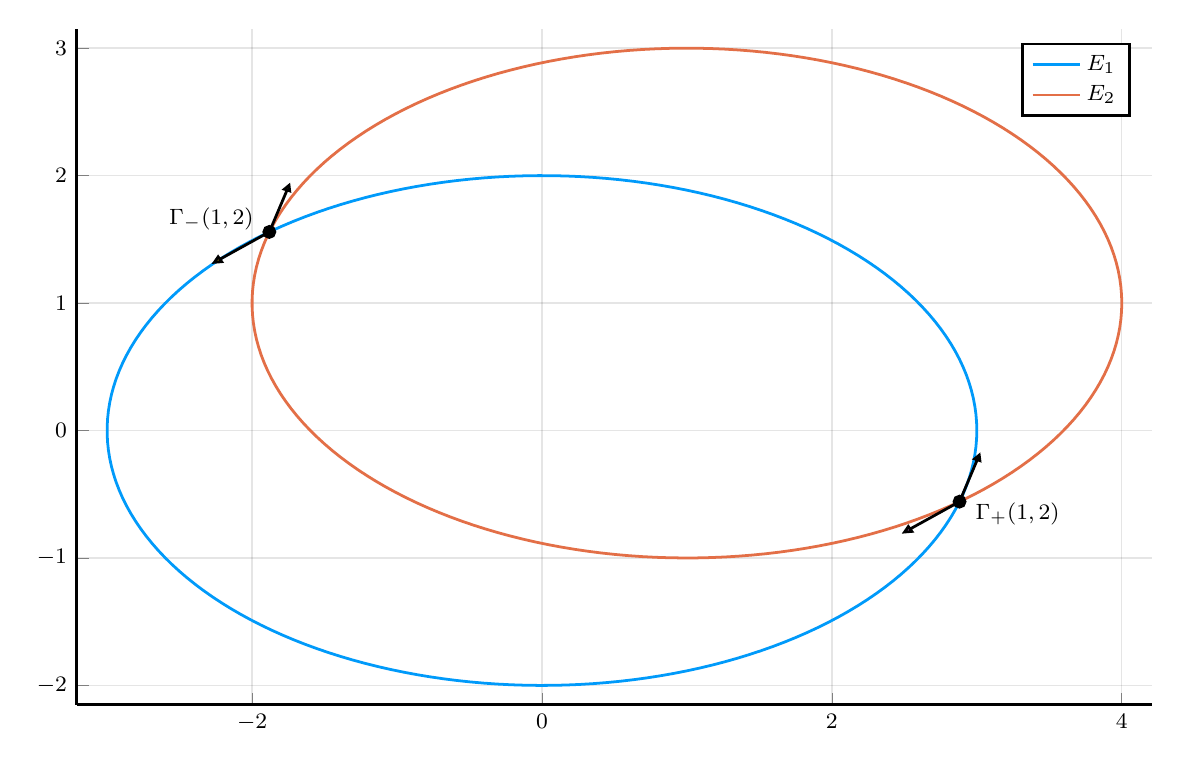
\begin{tikzpicture}[]
\begin{axis}[height = {101.6mm}, ylabel = {}, xmin = {-3.209614953609561}, xmax = {4.20998878505659}, ymax = {3.1499339554156114}, xlabel = {}, unbounded coords=jump,scaled x ticks = false,xlabel style = {font = {\fontsize{11 pt}{14.3 pt}\selectfont}, color = {rgb,1:red,0.00000000;green,0.00000000;blue,0.00000000}, draw opacity = 1.0, rotate = 0.0},xmajorgrids = true,xtick = {-2.0,0.0,2.0,4.0},xticklabels = {$-2$,$0$,$2$,$4$},xtick align = inside,xticklabel style = {font = {\fontsize{8 pt}{10.4 pt}\selectfont}, color = {rgb,1:red,0.00000000;green,0.00000000;blue,0.00000000}, draw opacity = 1.0, rotate = 0.0},x grid style = {color = {rgb,1:red,0.00000000;green,0.00000000;blue,0.00000000},
draw opacity = 0.1,
line width = 0.5,
solid},axis lines* = left,x axis line style = {color = {rgb,1:red,0.00000000;green,0.00000000;blue,0.00000000},
draw opacity = 1.0,
line width = 1,
solid},scaled y ticks = false,ylabel style = {font = {\fontsize{11 pt}{14.3 pt}\selectfont}, color = {rgb,1:red,0.00000000;green,0.00000000;blue,0.00000000}, draw opacity = 1.0, rotate = 0.0},ymajorgrids = true,ytick = {-2.0,-1.0,0.0,1.0,2.0,3.0},yticklabels = {$-2$,$-1$,$0$,$1$,$2$,$3$},ytick align = inside,yticklabel style = {font = {\fontsize{8 pt}{10.4 pt}\selectfont}, color = {rgb,1:red,0.00000000;green,0.00000000;blue,0.00000000}, draw opacity = 1.0, rotate = 0.0},y grid style = {color = {rgb,1:red,0.00000000;green,0.00000000;blue,0.00000000},
draw opacity = 0.1,
line width = 0.5,
solid},axis lines* = left,y axis line style = {color = {rgb,1:red,0.00000000;green,0.00000000;blue,0.00000000},
draw opacity = 1.0,
line width = 1,
solid},    xshift = 0.0mm,
    yshift = 0.0mm,
    axis background/.style={fill={rgb,1:red,1.00000000;green,1.00000000;blue,1.00000000}}
,legend style = {color = {rgb,1:red,0.00000000;green,0.00000000;blue,0.00000000},
draw opacity = 1.0,
line width = 1,
solid,fill = {rgb,1:red,1.00000000;green,1.00000000;blue,1.00000000},font = {\fontsize{8 pt}{10.4 pt}\selectfont}},colorbar style={title=}, ymin = {-2.1499339554156114}, width = {152.4mm}]\addplot+ [color = {rgb,1:red,0.00000000;green,0.60560316;blue,0.97868012},
draw opacity = 1.0,
line width = 1,
solid,mark = none,
mark size = 2.0,
mark options = {
    color = {rgb,1:red,0.00000000;green,0.00000000;blue,0.00000000}, draw opacity = 1.0,
    fill = {rgb,1:red,0.00000000;green,0.60560316;blue,0.97868012}, fill opacity = 1.0,
    line width = 1,
    rotate = 0,
    solid
}]coordinates {
(3.0, 0.0)
(2.9985047673785212, 0.06313709952962106)
(2.99402055999448, 0.1262112626253473)
(2.9865518478033177, 0.18915961558968988)
(2.9761060757797733, 0.2519194101354351)
(2.962693656496571, 0.31442808593450156)
(2.9463279597449414, 0.37662333297943573)
(2.9270252992073207, 0.43844315369538267)
(2.9048049161955216, 0.4998259247406167)
(2.879688960470571, 0.5607104584340288)
(2.8517024681633485, 0.6210360637483376)
(2.8208733368180265, 0.6807426068082256)
(2.787232297583192, 0.7397705708330936)
(2.7508128845783664, 0.7980611154646818)
(2.7116514014664705, 0.8555561354204192)
(2.669786885265541, 0.9121983184140319)
(2.625261067435781, 0.9679312022856775)
(2.578118332280736, 1.0226992312846535)
(2.528405672704052, 1.076447811448577)
(2.4761726433659286, 1.1291233650238361)
(2.421471311285956, 1.1806733838730568)
(2.3643562039415773, 1.2310464818163585)
(2.3048842549139126, 1.2801924458542142)
(2.2431147471351274, 1.3280622862208624)
(2.1791092537939183, 1.3746082852183685)
(2.1129315769580166, 1.4197840447826657)
(2.0446476839749015, 1.4635445327341534)
(1.974325641714113, 1.505846127666754)
(1.902035548716716, 1.546646662430678)
(1.82784946531955, 1.5859054661655572)
(1.7518413418239187, 1.6235834048420414)
(1.6740869447803206, 1.6596429202714515)
(1.5946637814627043, 1.6940480675445977)
(1.5136510226075326, 1.7267645508624465)
(1.4311294234946685, 1.7577597577229207)
(1.3471812434487604, 1.7870027914297482)
(1.261890163841353, 1.8144645018909626)
(1.1753412046754794, 1.840117514676349)
(1.0876206398358734, 1.8639362583048695)
(0.9988159110892831, 1.885896989734874)
(0.9090155409206182, 1.9059778180316784)
(0.8183090442918096, 1.9241587261889257)
(0.7267868394113495, 1.9404215910819727)
(0.6345401576034572, 1.9547502015334144)
(0.541660952366707, 1.9671302744727397)
(0.4482418077127828, 1.9775494691740052)
(0.35437584587672416, 1.9859973995573392)
(0.26015663449065285, 1.9924656445420135)
(0.1656780933135245, 1.9969477564407576)
(0.0710344006098723, 1.9994392673869559)
(-0.02368010072913993, 1.9999376937883127)
(-0.1183709972287581, 1.9984425388025513)
(-0.21294389894404733, 1.9949552928326777)
(-0.3073045335498399, 1.9894794320413138)
(-0.40135884031343716, 1.9820204148855842)
(-0.49501306385639726, 1.9725856766760055)
(-0.588173847611934, 1.9611846221648082)
(-0.68074832688477, 1.9478286161710756)
(-0.7726442214206901, 1.9325309722520436)
(-0.8637699273934991, 1.9153069394318591)
(-0.9540346087177143, 1.896173687001019)
(-1.043348287595947, 1.8751502874016501)
(-1.1316219342107279, 1.8522576972156826)
(-1.2187675554713666, 1.8275187362748735)
(-1.304698282727379, 1.8009580649135033)
(-1.389328458361043, 1.7726021593864174)
(-1.4725737211727805, 1.7424792854769193)
(-1.5543510904742317, 1.710619470320824)
(-1.6345790488052114, 1.6770544724747547)
(-1.713177623192084, 1.6418177502585252)
(-1.7900684648665677, 1.604944428403156)
(-1.8651749273654852, 1.566471263037781)
(-1.9384221429336286, 1.5264366050503373)
(-2.009737097153566, 1.484880361858566)
(-2.079048701727995, 1.4418439576294326)
(-2.1462878653421136, 1.3973702919866131)
(-2.2113875625353363, 1.3515036972472176)
(-2.274282900513736, 1.3042898942303736)
(-2.3349111838365904, 1.2557759466817167)
(-2.393211976912558, 1.206010214359229)
(-2.449127164243197, 1.1550423048271772)
(-2.502601008353752, 1.1029230240062151)
(-2.5535802053534837, 1.0497043255289369)
(-2.6020139380701437, 0.9954392589513668)
(-2.6478539267056407, 0.9401819168720059)
(-2.6910544769623908, 0.8839873810111583)
(-2.7315725255923864, 0.8269116673042683)
(-2.7693676833235816, 0.769011670064022)
(-2.8044022751207947, 0.7103451052668572)
(-2.8366413777410013, 0.6509704530204232)
(-2.8660528545455843, 0.5909468992693401)
(-2.8926073875348353, 0.5303342767973575)
(-2.916278506572771, 0.46919300558473775)
(-2.9370426157731435, 0.4075840325803047)
(-2.954879017020331, 0.3455687709481997)
(-2.9697699306016716, 0.28320903884990317)
(-2.9817005129306633, 0.22056699782255015)
(-2.9906588713433795, 0.1577050908149532)
(-2.996636075953331, 0.09468597994311641)
(-2.9996261685529717, 0.03157248402727453)
(-2.9996261685529717, -0.031572484027274035)
(-2.996636075953331, -0.09468597994311592)
(-2.9906588713433795, -0.1577050908149527)
(-2.9817005129306637, -0.22056699782254965)
(-2.9697699306016716, -0.2832090388499027)
(-2.9548790170203314, -0.34556877094819927)
(-2.9370426157731435, -0.40758403258030423)
(-2.916278506572771, -0.46919300558473725)
(-2.8926073875348353, -0.530334276797357)
(-2.866052854545585, -0.5909468992693396)
(-2.8366413777410013, -0.6509704530204228)
(-2.804402275120795, -0.7103451052668568)
(-2.769367683323582, -0.7690116700640215)
(-2.7315725255923864, -0.8269116673042679)
(-2.6910544769623908, -0.8839873810111578)
(-2.647853926705641, -0.9401819168720055)
(-2.6020139380701437, -0.9954392589513663)
(-2.5535802053534837, -1.0497043255289367)
(-2.5026010083537527, -1.1029230240062147)
(-2.4491271642431975, -1.155042304827177)
(-2.393211976912559, -1.2060102143592286)
(-2.3349111838365904, -1.2557759466817162)
(-2.274282900513737, -1.3042898942303731)
(-2.211387562535337, -1.3515036972472174)
(-2.1462878653421145, -1.3973702919866127)
(-2.079048701727996, -1.4418439576294324)
(-2.0097370971535664, -1.4848803618585658)
(-1.9384221429336304, -1.5264366050503364)
(-1.8651749273654858, -1.5664712630377808)
(-1.7900684648665695, -1.604944428403155)
(-1.713177623192085, -1.641817750258525)
(-1.634579048805211, -1.677054472474755)
(-1.5543510904742333, -1.7106194703208233)
(-1.4725737211727812, -1.742479285476919)
(-1.389328458361045, -1.7726021593864167)
(-1.3046982827273796, -1.800958064913503)
(-1.2187675554713666, -1.8275187362748735)
(-1.131621934210729, -1.8522576972156821)
(-1.0433482875959472, -1.8751502874016501)
(-0.9540346087177163, -1.8961736870010186)
(-0.8637699273935, -1.915306939431859)
(-0.7726442214206894, -1.9325309722520438)
(-0.6807483268847714, -1.9478286161710754)
(-0.5881738476119341, -1.9611846221648082)
(-0.4950130638563993, -1.9725856766760053)
(-0.4013588403134378, -1.9820204148855842)
(-0.3073045335498393, -1.989479432041314)
(-0.2129438989440487, -1.9949552928326775)
(-0.11837099722875816, -1.9984425388025513)
(-0.023680100729141333, -1.9999376937883127)
(0.07103440060987157, -1.9994392673869559)
(0.1656780933135251, -1.9969477564407576)
(0.2601566344906514, -1.9924656445420135)
(0.3543758458767241, -1.9859973995573392)
(0.44824180771278144, -1.9775494691740052)
(0.5416609523667063, -1.96713027447274)
(0.6345401576034577, -1.9547502015334144)
(0.7267868394113488, -1.9404215910819727)
(0.8183090442918095, -1.9241587261889257)
(0.9090155409206169, -1.9059778180316789)
(0.998815911089283, -1.885896989734874)
(1.0876206398358716, -1.8639362583048702)
(1.1753412046754788, -1.840117514676349)
(1.261890163841353, -1.8144645018909626)
(1.3471812434487593, -1.7870027914297486)
(1.4311294234946685, -1.7577597577229207)
(1.5136510226075308, -1.7267645508624474)
(1.5946637814627036, -1.694048067544598)
(1.6740869447803208, -1.6596429202714515)
(1.7518413418239178, -1.6235834048420419)
(1.82784946531955, -1.5859054661655572)
(1.9020355487167147, -1.546646662430679)
(1.9743256417141124, -1.5058461276667543)
(2.044647683974902, -1.4635445327341534)
(2.1129315769580157, -1.4197840447826664)
(2.179109253793918, -1.3746082852183685)
(2.243114747135126, -1.3280622862208633)
(2.3048842549139117, -1.2801924458542147)
(2.3643562039415773, -1.231046481816358)
(2.4214713112859556, -1.1806733838730574)
(2.4761726433659286, -1.1291233650238361)
(2.528405672704051, -1.076447811448578)
(2.5781183322807357, -1.0226992312846537)
(2.6252610674357815, -0.9679312022856771)
(2.66978688526554, -0.9121983184140325)
(2.7116514014664705, -0.8555561354204191)
(2.750812884578366, -0.7980611154646828)
(2.7872322975831914, -0.7397705708330939)
(2.820873336818026, -0.680742606808227)
(2.8517024681633485, -0.6210360637483382)
(2.879688960470571, -0.5607104584340287)
(2.904804916195521, -0.4998259247406176)
(2.9270252992073207, -0.4384431536953829)
(2.946327959744941, -0.37662333297943695)
(2.9626936564965707, -0.3144280859345021)
(2.9761060757797737, -0.25191941013543495)
(2.9865518478033177, -0.18915961558969077)
(2.99402055999448, -0.12621126262534743)
(2.9985047673785212, -0.06313709952962226)
(3.0, -4.898587196589413e-16)
};
\addlegendentry{$E_1$}
\addplot+ [color = {rgb,1:red,0.88887350;green,0.43564919;blue,0.27812294},
draw opacity = 1.0,
line width = 1,
solid,mark = none,
mark size = 2.0,
mark options = {
    color = {rgb,1:red,0.00000000;green,0.00000000;blue,0.00000000}, draw opacity = 1.0,
    fill = {rgb,1:red,0.88887350;green,0.43564919;blue,0.27812294}, fill opacity = 1.0,
    line width = 1,
    rotate = 0,
    solid
}]coordinates {
(4.0, 1.0)
(3.9985047673785212, 1.063137099529621)
(3.99402055999448, 1.1262112626253473)
(3.9865518478033177, 1.18915961558969)
(3.9761060757797733, 1.2519194101354352)
(3.962693656496571, 1.3144280859345017)
(3.9463279597449414, 1.3766233329794357)
(3.9270252992073207, 1.4384431536953826)
(3.9048049161955216, 1.4998259247406167)
(3.879688960470571, 1.5607104584340288)
(3.8517024681633485, 1.6210360637483376)
(3.8208733368180265, 1.6807426068082256)
(3.787232297583192, 1.7397705708330937)
(3.7508128845783664, 1.798061115464682)
(3.7116514014664705, 1.8555561354204193)
(3.669786885265541, 1.9121983184140319)
(3.625261067435781, 1.9679312022856776)
(3.578118332280736, 2.0226992312846535)
(3.528405672704052, 2.0764478114485767)
(3.4761726433659286, 2.129123365023836)
(3.421471311285956, 2.1806733838730565)
(3.3643562039415773, 2.2310464818163585)
(3.3048842549139126, 2.2801924458542144)
(3.2431147471351274, 2.328062286220862)
(3.1791092537939183, 2.3746082852183683)
(3.1129315769580166, 2.4197840447826655)
(3.0446476839749015, 2.4635445327341534)
(2.9743256417141133, 2.505846127666754)
(2.902035548716716, 2.5466466624306783)
(2.82784946531955, 2.585905466165557)
(2.7518413418239187, 2.6235834048420417)
(2.6740869447803206, 2.6596429202714518)
(2.594663781462704, 2.694048067544598)
(2.5136510226075326, 2.7267645508624465)
(2.4311294234946685, 2.757759757722921)
(2.3471812434487607, 2.787002791429748)
(2.261890163841353, 2.8144645018909626)
(2.1753412046754796, 2.840117514676349)
(2.0876206398358734, 2.8639362583048698)
(1.9988159110892831, 2.8858969897348743)
(1.9090155409206182, 2.9059778180316784)
(1.8183090442918095, 2.9241587261889257)
(1.7267868394113495, 2.9404215910819724)
(1.6345401576034573, 2.9547502015334146)
(1.541660952366707, 2.9671302744727397)
(1.4482418077127828, 2.977549469174005)
(1.354375845876724, 2.9859973995573394)
(1.2601566344906527, 2.9924656445420137)
(1.1656780933135245, 2.9969477564407576)
(1.0710344006098722, 2.999439267386956)
(0.97631989927086, 2.9999376937883127)
(0.8816290027712419, 2.9984425388025513)
(0.7870561010559527, 2.9949552928326777)
(0.6926954664501601, 2.989479432041314)
(0.5986411596865628, 2.982020414885584)
(0.5049869361436028, 2.9725856766760055)
(0.41182615238806597, 2.961184622164808)
(0.31925167311522995, 2.9478286161710754)
(0.2273557785793099, 2.9325309722520436)
(0.13623007260650088, 2.915306939431859)
(0.04596539128228572, 2.896173687001019)
(-0.043348287595947, 2.87515028740165)
(-0.13162193421072788, 2.8522576972156823)
(-0.21876755547136661, 2.8275187362748735)
(-0.304698282727379, 2.8009580649135035)
(-0.389328458361043, 2.7726021593864174)
(-0.4725737211727805, 2.7424792854769193)
(-0.5543510904742317, 2.710619470320824)
(-0.6345790488052114, 2.6770544724747545)
(-0.7131776231920841, 2.641817750258525)
(-0.7900684648665677, 2.604944428403156)
(-0.8651749273654852, 2.566471263037781)
(-0.9384221429336286, 2.5264366050503373)
(-1.009737097153566, 2.4848803618585658)
(-1.079048701727995, 2.4418439576294326)
(-1.1462878653421136, 2.397370291986613)
(-1.2113875625353363, 2.3515036972472174)
(-1.274282900513736, 2.3042898942303736)
(-1.3349111838365904, 2.255775946681717)
(-1.393211976912558, 2.206010214359229)
(-1.449127164243197, 2.155042304827177)
(-1.5026010083537522, 2.1029230240062153)
(-1.5535802053534837, 2.049704325528937)
(-1.6020139380701437, 1.9954392589513668)
(-1.6478539267056407, 1.9401819168720058)
(-1.6910544769623908, 1.8839873810111583)
(-1.7315725255923864, 1.8269116673042682)
(-1.7693676833235816, 1.769011670064022)
(-1.8044022751207947, 1.7103451052668572)
(-1.8366413777410013, 1.6509704530204232)
(-1.8660528545455843, 1.59094689926934)
(-1.8926073875348353, 1.5303342767973573)
(-1.916278506572771, 1.4691930055847378)
(-1.9370426157731435, 1.4075840325803046)
(-1.954879017020331, 1.3455687709481996)
(-1.9697699306016716, 1.2832090388499031)
(-1.9817005129306633, 1.2205669978225502)
(-1.9906588713433795, 1.1577050908149533)
(-1.9966360759533308, 1.0946859799431163)
(-1.9996261685529717, 1.0315724840272744)
(-1.9996261685529717, 0.9684275159727259)
(-1.9966360759533308, 0.9053140200568841)
(-1.9906588713433795, 0.8422949091850473)
(-1.9817005129306637, 0.7794330021774504)
(-1.9697699306016716, 0.7167909611500973)
(-1.9548790170203314, 0.6544312290518007)
(-1.9370426157731435, 0.5924159674196958)
(-1.916278506572771, 0.5308069944152627)
(-1.8926073875348353, 0.469665723202643)
(-1.8660528545455848, 0.40905310073066037)
(-1.8366413777410013, 0.3490295469795772)
(-1.804402275120795, 0.2896548947331432)
(-1.769367683323582, 0.2309883299359785)
(-1.7315725255923864, 0.1730883326957321)
(-1.6910544769623908, 0.11601261898884219)
(-1.6478539267056411, 0.059818083127994526)
(-1.6020139380701437, 0.0045607410486336875)
(-1.5535802053534837, -0.049704325528936666)
(-1.5026010083537527, -0.10292302400621467)
(-1.4491271642431975, -0.15504230482717696)
(-1.3932119769125588, -0.20601021435922862)
(-1.3349111838365904, -0.2557759466817162)
(-1.2742829005137368, -0.3042898942303731)
(-1.2113875625353372, -0.3515036972472174)
(-1.1462878653421145, -0.39737029198661267)
(-1.079048701727996, -0.4418439576294324)
(-1.0097370971535664, -0.48488036185856576)
(-0.9384221429336304, -0.5264366050503364)
(-0.8651749273654858, -0.5664712630377808)
(-0.7900684648665695, -0.6049444284031551)
(-0.713177623192085, -0.6418177502585249)
(-0.634579048805211, -0.6770544724747549)
(-0.5543510904742333, -0.7106194703208233)
(-0.4725737211727812, -0.7424792854769191)
(-0.389328458361045, -0.7726021593864167)
(-0.30469828272737964, -0.8009580649135031)
(-0.21876755547136661, -0.8275187362748735)
(-0.13162193421072899, -0.8522576972156821)
(-0.04334828759594722, -0.8751502874016501)
(0.04596539128228372, -0.8961736870010186)
(0.1362300726065, -0.9153069394318589)
(0.22735577857931055, -0.9325309722520438)
(0.3192516731152286, -0.9478286161710754)
(0.41182615238806586, -0.9611846221648082)
(0.5049869361436007, -0.9725856766760053)
(0.5986411596865622, -0.9820204148855842)
(0.6926954664501608, -0.989479432041314)
(0.7870561010559514, -0.9949552928326775)
(0.8816290027712419, -0.9984425388025513)
(0.9763198992708587, -0.9999376937883127)
(1.0710344006098715, -0.9994392673869559)
(1.1656780933135251, -0.9969477564407576)
(1.2601566344906514, -0.9924656445420135)
(1.354375845876724, -0.9859973995573392)
(1.4482418077127814, -0.9775494691740052)
(1.5416609523667062, -0.9671302744727399)
(1.6345401576034577, -0.9547502015334144)
(1.7267868394113488, -0.9404215910819727)
(1.8183090442918095, -0.9241587261889257)
(1.9090155409206169, -0.9059778180316789)
(1.9988159110892831, -0.8858969897348741)
(2.0876206398358716, -0.8639362583048702)
(2.1753412046754788, -0.8401175146763491)
(2.261890163841353, -0.8144645018909626)
(2.3471812434487593, -0.7870027914297486)
(2.4311294234946685, -0.7577597577229207)
(2.513651022607531, -0.7267645508624474)
(2.5946637814627036, -0.6940480675445979)
(2.6740869447803206, -0.6596429202714515)
(2.751841341823918, -0.6235834048420419)
(2.82784946531955, -0.5859054661655572)
(2.9020355487167144, -0.5466466624306789)
(2.9743256417141124, -0.5058461276667543)
(3.044647683974902, -0.4635445327341534)
(3.1129315769580157, -0.4197840447826664)
(3.179109253793918, -0.37460828521836853)
(3.243114747135126, -0.3280622862208633)
(3.3048842549139117, -0.28019244585421466)
(3.3643562039415773, -0.231046481816358)
(3.4214713112859556, -0.18067338387305742)
(3.4761726433659286, -0.12912336502383615)
(3.528405672704051, -0.07644781144857804)
(3.5781183322807357, -0.022699231284653676)
(3.6252610674357815, 0.032068797714322916)
(3.66978688526554, 0.08780168158596746)
(3.7116514014664705, 0.14444386457958092)
(3.750812884578366, 0.20193888453531716)
(3.7872322975831914, 0.26022942916690606)
(3.820873336818026, 0.31925739319177304)
(3.8517024681633485, 0.3789639362516618)
(3.879688960470571, 0.43928954156597133)
(3.904804916195521, 0.5001740752593824)
(3.9270252992073207, 0.5615568463046171)
(3.946327959744941, 0.623376667020563)
(3.9626936564965707, 0.6855719140654979)
(3.9761060757797737, 0.748080589864565)
(3.9865518478033177, 0.8108403844103093)
(3.99402055999448, 0.8737887373746526)
(3.9985047673785212, 0.9368629004703777)
(4.0, 0.9999999999999996)
};
\addlegendentry{$E_2$}
\addplot+[draw=none, color = {rgb,1:red,0.00000000;green,0.00000000;blue,0.00000000},
draw opacity = 1.0,
line width = 0,
solid,mark = *,
mark size = 2.0,
mark options = {
    color = {rgb,1:red,0.00000000;green,0.00000000;blue,0.00000000}, draw opacity = 1.0,
    fill = {rgb,1:red,0.00000000;green,0.00000000;blue,0.00000000}, fill opacity = 1.0,
    line width = 1,
    rotate = 0,
    solid
},forget plot] coordinates {
(2.880812724841925, -0.5581389888186332)
(-1.8808127248419249, 1.5581389888186332)
};
\addplot+ [color = {rgb,1:red,0.00000000;green,0.00000000;blue,0.00000000},
draw opacity = 1.0,
line width = 1,
solid,mark = none,
mark size = 2.0,
mark options = {
    color = {rgb,1:red,0.00000000;green,0.00000000;blue,0.00000000}, draw opacity = 1.0,
    fill = {rgb,1:red,0.76444018;green,0.44411178;blue,0.82429754}, fill opacity = 1.0,
    line width = 1,
    rotate = 0,
    solid
},fill = {rgb,1:red,0.76444018;green,0.44411178;blue,0.82429754}, fill opacity=1.0,forget plot]coordinates {
(2.880812724841925, -0.5581389888186332)
(3.003063448757894, -0.22957188356452582)
(2.9848097206882214, -0.2227801766803053)
(3.016646862526335, -0.19306442742518054)
(3.0213171768275666, -0.23636359044874633)
(3.003063448757894, -0.22957188356452582)
};
\addplot+ [color = {rgb,1:red,0.00000000;green,0.00000000;blue,0.00000000},
draw opacity = 1.0,
line width = 1,
solid,mark = none,
mark size = 2.0,
mark options = {
    color = {rgb,1:red,0.00000000;green,0.00000000;blue,0.00000000}, draw opacity = 1.0,
    fill = {rgb,1:red,0.76444018;green,0.44411178;blue,0.82429754}, fill opacity = 1.0,
    line width = 1,
    rotate = 0,
    solid
},fill = {rgb,1:red,0.76444018;green,0.44411178;blue,0.82429754}, fill opacity=1.0,forget plot]coordinates {
(2.880812724841925, -0.5581389888186332)
(2.5395292396155034, -0.7726524791255432)
(2.551446655743665, -0.7916126727492333)
(2.5016088523681232, -0.7964873113818666)
(2.5276118234873417, -0.7536922855018532)
(2.5395292396155034, -0.7726524791255432)
};
\addplot+ [color = {rgb,1:red,0.00000000;green,0.00000000;blue,0.00000000},
draw opacity = 1.0,
line width = 1,
solid,mark = none,
mark size = 2.0,
mark options = {
    color = {rgb,1:red,0.00000000;green,0.00000000;blue,0.00000000}, draw opacity = 1.0,
    fill = {rgb,1:red,0.67554396;green,0.55566233;blue,0.09423434}, fill opacity = 1.0,
    line width = 1,
    rotate = 0,
    solid
},fill = {rgb,1:red,0.67554396;green,0.55566233;blue,0.09423434}, fill opacity=1.0,forget plot]coordinates {
(-1.8808127248419249, 1.5581389888186332)
(-2.2220962100683463, 1.3436254985117233)
(-2.2101787939401847, 1.3246653048880332)
(-2.2600165973157265, 1.3197906662554)
(-2.234013626196508, 1.3625856921354134)
(-2.2220962100683463, 1.3436254985117233)
};
\addplot+ [color = {rgb,1:red,0.00000000;green,0.00000000;blue,0.00000000},
draw opacity = 1.0,
line width = 1,
solid,mark = none,
mark size = 2.0,
mark options = {
    color = {rgb,1:red,0.00000000;green,0.00000000;blue,0.00000000}, draw opacity = 1.0,
    fill = {rgb,1:red,0.67554396;green,0.55566233;blue,0.09423434}, fill opacity = 1.0,
    line width = 1,
    rotate = 0,
    solid
},fill = {rgb,1:red,0.67554396;green,0.55566233;blue,0.09423434}, fill opacity=1.0,forget plot]coordinates {
(-1.8808127248419249, 1.5581389888186332)
(-1.758562000925956, 1.8867060940727407)
(-1.7768157289956286, 1.8934978009569612)
(-1.744978587157515, 1.923213550212086)
(-1.7403082728562833, 1.8799143871885202)
(-1.758562000925956, 1.8867060940727407)
};
\node at (axis cs:3.2808127248419248, -0.6581389888186332) [,
color={rgb,1:red,0.00000000;green,0.00000000;blue,0.00000000}, draw opacity=1.0,
rotate=0.0,
font={\fontsize{8 pt}{10.4 pt}\selectfont}
] {$\tiny\Gamma_+(1,2)$};
\node at (axis cs:-2.2808127248419248, 1.6581389888186333) [,
color={rgb,1:red,0.00000000;green,0.00000000;blue,0.00000000}, draw opacity=1.0,
rotate=0.0,
font={\fontsize{8 pt}{10.4 pt}\selectfont}
] {$\tiny\Gamma_-(1,2)$};
\end{axis}

\end{tikzpicture}

		%\fautor
		\label{fig:3ellipses_intersect}
	\end{figure}
\end{frame}

\section{Maximal Covering by Disks}
\begin{frame}{Maximal Covering by Disks}{One disk}
	
	$MCD(\Pp, 1)$ is the problem of placing one disk on the plane to cover a subset of a demand set $\Pp$ maximizing the weights of the covered points.
	
	\begin{equation*}\label{eq:max_one_disk}
		\max_q w(\Pp \cap D(q)),
	\end{equation*}
	
	\begin{itemize}
		\item $\Pp=\{p_1,\dots,p_n\}$ is the demand set with weights $w(p_i)>0$
		\item $w(A)$, with $A\subset \Pp$ is the sum of weights of the points in $A$
		\item $D(q)$ is a disk with radius one with center at point $q$
		\item We will introduce an equivalent problem...
	\end{itemize}
\end{frame}

\subsection{Maximum Weight Clique Problem}
\begin{frame}{Maximum Weight Clique Problem}
	Let $\D=\{D_1,\dots,D_n\}$ be a set of $n$ unit disks with weights $w_i>0$. The maximum weight clique is defined as
	
	\begin{equation*}
	\max_q \sum_{D_k \cap q \neq \emptyset} w_k,
	\end{equation*}
	
	\begin{itemize}
		\item The disks are fixed at $\Pp =\{p_1,\dots,p_n\}$ with $w_k=w(p_k)$
		\item A clique is a non-empty intersection area of a subset of disks
		\item An optimal solution for the maximum weight clique is an optimal solution for $MCD(\Pp,1)$.
	\end{itemize}
\end{frame}


\section{Cobertura Maximal por Ellipses}

\begin{frame}{Cobertura Maximal por Ellipses}
	content... trabalhos passados
\end{frame}

\begin{frame}{Cobertura Maximal por Ellipses}{$m$ elipses}
	content... algoritmo
\end{frame}

\section{Trabalhos Futuros}

\begin{frame}{Trabalhos Futuros}

\end{frame}
\end{document}